\documentclass{beamer}
\usepackage{gb4e}
\usepackage{tikz}
\usepackage{color}
\usepackage{array}
\usepackage{multirow}
\usepackage{booktabs}
\usepackage{hyperref}

\newcommand{\corpus}[1]{\textit{#1}}

%Information to be included in the title page:
\title{Family trees of languages}
\author{Jinyuan Wu}

\usetheme{Madrid}

\begin{document}

\frame{\titlepage}

\begin{frame}
\frametitle{Introduction}

We know how a family evolves.

\begin{center}
    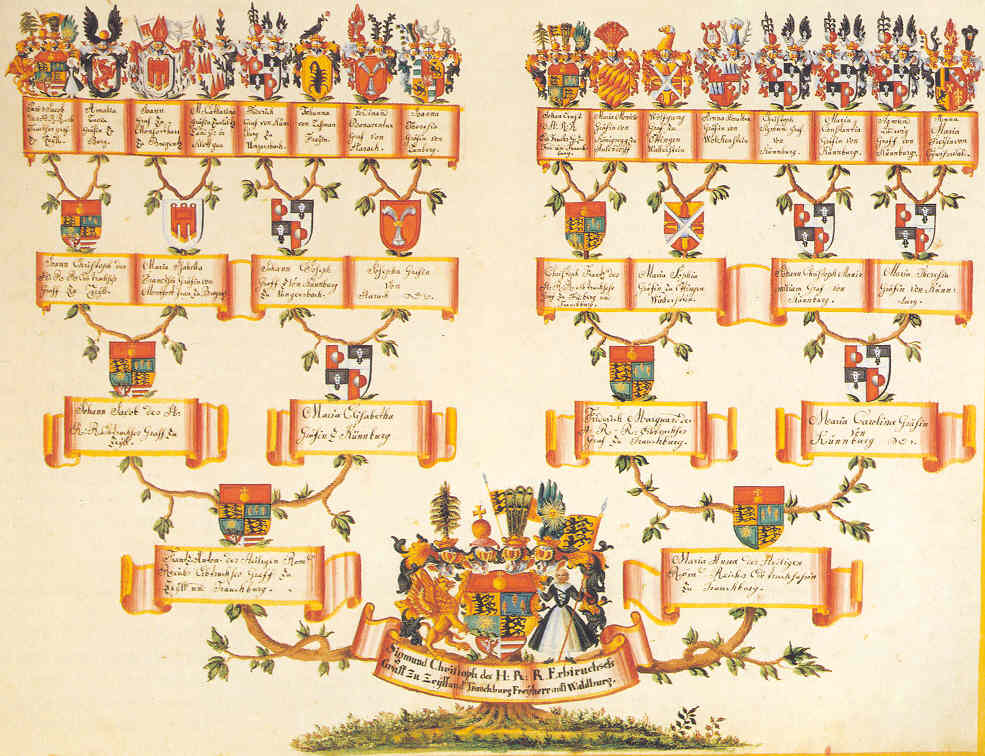
\includegraphics[width=0.6\textwidth]{photos/Waldburg-Ahnentafel.jpg}
\end{center} 

But what about languages?

\end{frame}

\begin{frame}
\frametitle{Languages evolve in their own ways}

``\textbf{Neogrammarian hypothesis}'':
word changes can only arise from
\begin{itemize}
    \item Regular sound laws: \corpus{p} $>$ \corpus{f} (in \emph{all} words as long as the sound is in the correct environment!)
    \item Borrowing: Arabic \corpus{ṣuffa} $>$ French \corpus{sofa} $>$ English \corpus{sofa} $>$ Mandarin Chinese \corpus{sh\={a}f\={a}} 
    \item Analogy (self-regularization): do you know once people said \corpus{baken} instead of \corpus{baked}?
\end{itemize}    

\textbf{The tree model of language evolution}

\end{frame}

\begin{frame}
\frametitle{The comparative method}

    

\end{frame}

\begin{frame}
\frametitle{Some family trees}

    

\end{frame}

\end{document}